\documentclass[11pt]{article}
\usepackage[T1]{fontenc}
\usepackage[utf8]{inputenc}
\usepackage[letterpaper]{geometry}

\usepackage{graphicx}
\usepackage{mathpazo}

\usepackage{amsmath}
\usepackage{amsfonts}
\usepackage{bm}
\usepackage{siunitx}
\usepackage{cancel}
\usepackage{float}
\usepackage{empheq}
\usepackage[most]{tcolorbox}

% Sexy yellow highlighted boxed equations!
\newtcbox{\mymath}[1][]{%
	nobeforeafter, math upper, tcbox raise base,
	enhanced, colframe=black!30!black,
	colback=yellow!30, boxrule=1pt,
	#1}

% Hyperlinks with decent looking default colors.
\usepackage{hyperref}
\usepackage{xcolor}
\hypersetup{
	colorlinks,
	linkcolor={red!50!black},
	citecolor={blue!50!black},
	urlcolor={blue!80!black}
}

% For those sexy spaced low small caps from classic-thesis!
\usepackage{microtype}
\usepackage{textcase}
\DeclareRobustCommand{\spacedlowsmallcaps}[1]{%
	\textls[80]{\scshape\MakeTextLowercase{#1}}%
}

% Replaced mathpazo \sum symbol with computer modern's.
\DeclareSymbolFont{cmlargesymbols}{OMX}{cmex}{m}{n}
\let\sumop\relax
\DeclareMathSymbol{\sumop}{\mathop}{cmlargesymbols}{"50}

% Force indent command.
\newcommand{\forceindent}{\leavevmode{\parindent=1em\indent}}

% Math shortcuts.
\newcommand\p[2]{\frac{\partial #1}{\partial #2}}

% fancyhdr header and footer.
\usepackage{fancyhdr}
\pagestyle{fancy} 
\fancyhead{}
\rhead{Ali Ramadhan}
\chead{}
\lhead{12.818: Project 6}
\cfoot{}
\rfoot{\thepage}

\title{\spacedlowsmallcaps{\small 12.818: Introduction to Atmospheric Data and Large-scale Dynamics}\\ \spacedlowsmallcaps{\large Project seven: The Quasi-geostrophic Vorticity Equation}}
\author{\spacedlowsmallcaps{Ali Ramadhan}}
\date{}

\begin{document}
\maketitle

In this project we will study synoptic systems by employing the \emph{quasi-geostrophic vorticity equation}, which can be expressed mathematically in pressure coordinates as
\begin{equation*}
  \frac{D_g}{Dt}(\zeta_g + f) = -f (\nabla \cdot \bm{v}) = f\p{\omega}{p}
  = \frac{f}{\varrho} \p{(\varrho w)}{z}
\end{equation*}
where
\begin{equation*}
  \frac{D_g}{Dt} = \frac{\partial}{\partial t} + \bm{v}_g \cdot \nabla
\end{equation*}
is the geostrophic derivative operator, $\zeta_g + f$ is the absolute vorticity, $f$ is the planetary vorticity, $\zeta_g$ is the geostrophic relative vorticity evaluated on an isobaric surface, $\omega$ is the vertical velocity in pressure coordinates, $w$ is the vertical velocity in height coordinates, $\bm{v}$ is the wind velocity field, and $\bm{v}_g$ is the geostrophic wind velocity field.

Flows in \emph{quasi-geostrophic motion} have the Coriolis force and pressure  gradient forces \emph{almost} balancing each other, with interia providing the residual effect, as opposed to geostrophic balance where the Coriolis and pressure gradient forces are exactly in balance.

The quasi-geostrophic equation exhibits some useful properties. One is that it states that the sum of the relative, planetary, and stretching vorticities must be conserved following geostrophic motions. Another is that it allows for the determination of the geostrophic wind velocity and temperature fields from knowledge of the geopotential height only. Furthermore, if the time evolution of the geopotential height field is also known, vertical motions in the atmosphere may be inferred.

Note that positive vorticity is associated with low pressure systems, while negative vorticity is associated with high pressure systems.

Also note that the local rate of change of geostrophic vorticity is determined by the sum of two terms; the advection of the absolute vorticity by the geostrophic wind, and the the stretching or shrinking of fluid columns via a  divergence.

\section{Quasi-geostrophic scaling}

\begin{figure}[h!]
  \centering
  % trim={0 0 3.5cm 0}, clip,
  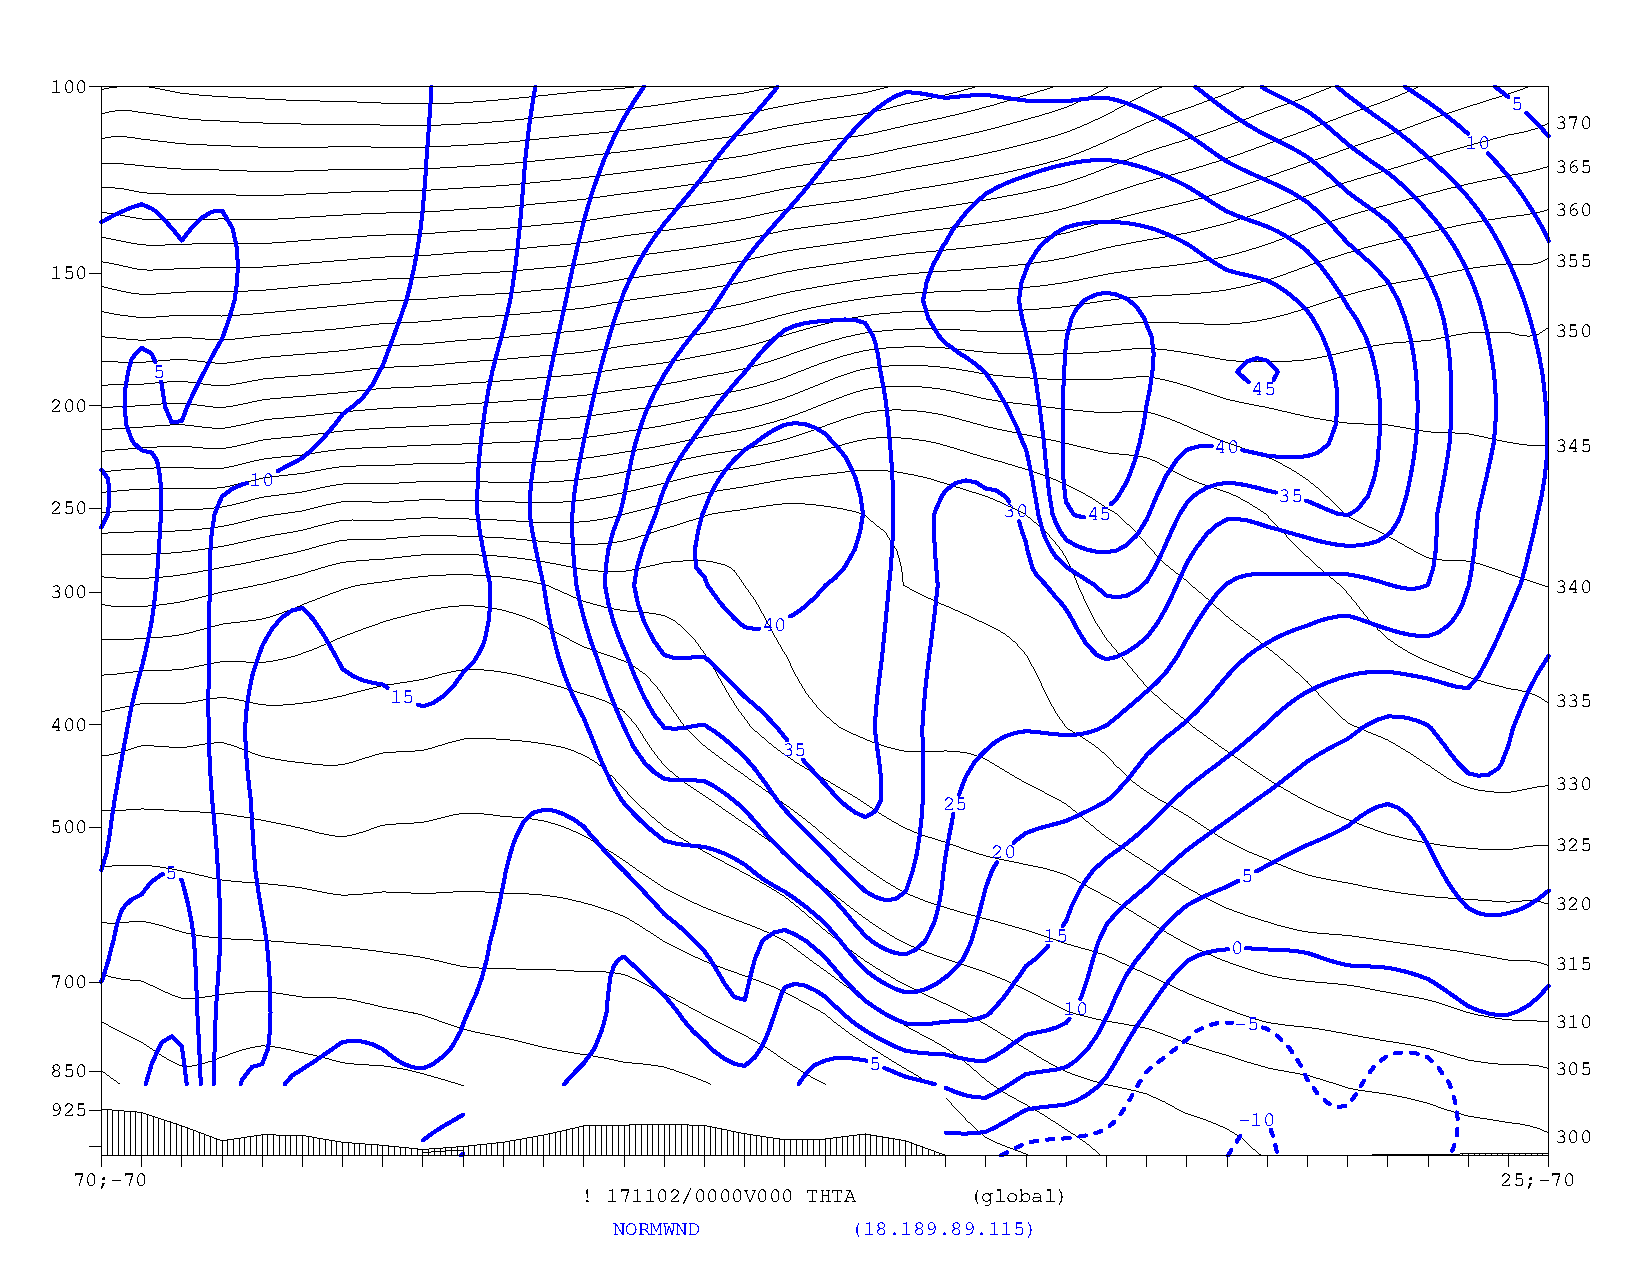
\includegraphics[width=\textwidth]{thta_normwnd_70W_25-70N}
  \caption{Meridional cross-section of the potential temperature (K) and observed wind velocity (normal to the cross-section) from \SI{25}{\degree N} to \SI{70}{\degree N} along the \SI{70}{\degree W} meridian (chosen to pass through Boston, MA) on November 2, 2017 (0Z).}
  \label{fig:thta_normwnd_mer_xsec}
\end{figure}

\begin{figure}[h!]
  \centering
  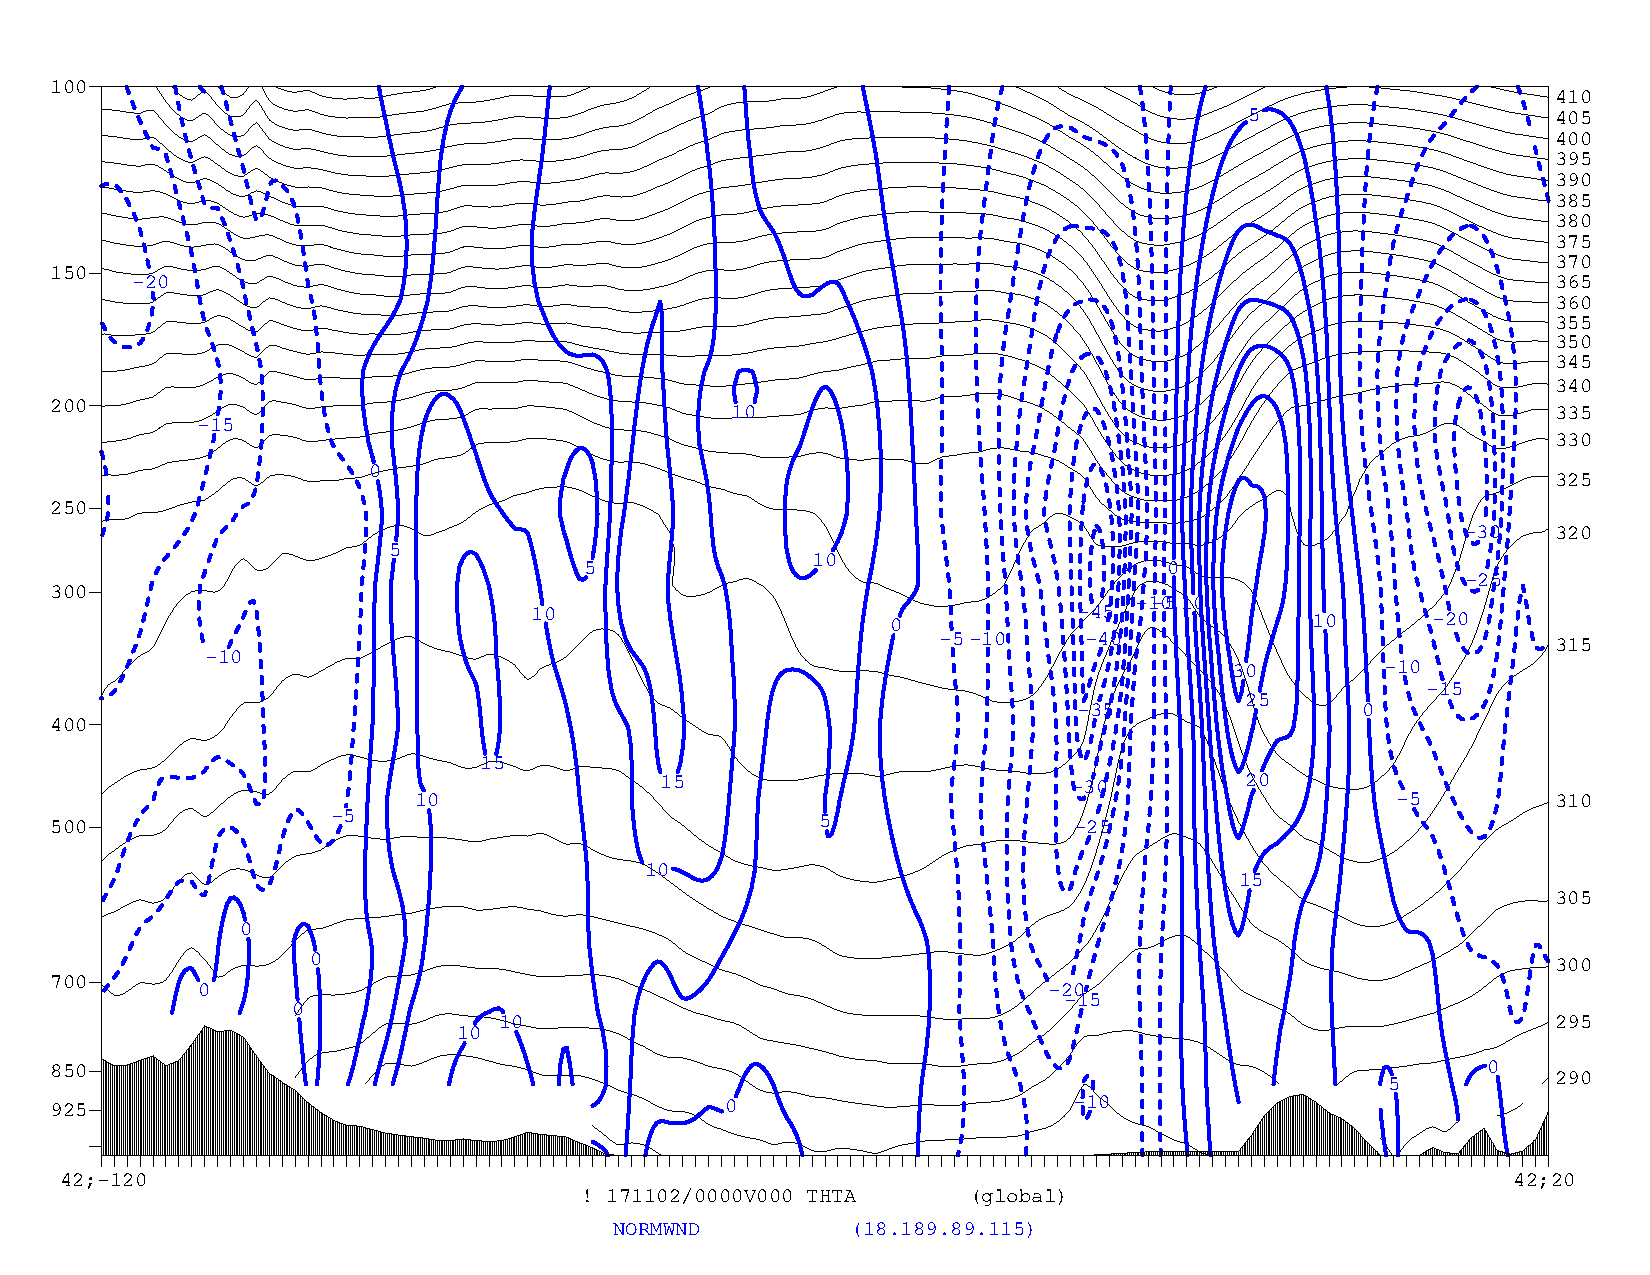
\includegraphics[width=\textwidth]{thta_normwnd_42N_120W-20E}
  \caption{Zonal cross-section of the potential temperature (K) and observed wind velocity (normal to the cross-section) from \SI{120}{\degree W} to \SI{20}{\degree E} along the \SI{42}{\degree N} meridian (chosen to pass through Boston, MA) on November 2, 2017 (0Z).}
  \label{fig:thta_normwnd_zon_xsec}
\end{figure}

\section{The Quasi-geostrophic vorticity equation}

\section{The Brunt--Väisälä frequency}

\end{document}